\documentclass[twoside]{book}

% Packages required by doxygen
\usepackage{fixltx2e}
\usepackage{calc}
\usepackage{doxygen}
\usepackage[export]{adjustbox} % also loads graphicx
\usepackage{graphicx}
\usepackage[utf8]{inputenc}
\usepackage{makeidx}
\usepackage{multicol}
\usepackage{multirow}
\PassOptionsToPackage{warn}{textcomp}
\usepackage{textcomp}
\usepackage[nointegrals]{wasysym}
\usepackage[table]{xcolor}

% Font selection
\usepackage[T1]{fontenc}
\usepackage[scaled=.90]{helvet}
\usepackage{courier}
\usepackage{amssymb}
\usepackage{sectsty}
\renewcommand{\familydefault}{\sfdefault}
\allsectionsfont{%
  \fontseries{bc}\selectfont%
  \color{darkgray}%
}
\renewcommand{\DoxyLabelFont}{%
  \fontseries{bc}\selectfont%
  \color{darkgray}%
}
\newcommand{\+}{\discretionary{\mbox{\scriptsize$\hookleftarrow$}}{}{}}

% Page & text layout
\usepackage{geometry}
\geometry{%
  a4paper,%
  top=2.5cm,%
  bottom=2.5cm,%
  left=2.5cm,%
  right=2.5cm%
}
\tolerance=750
\hfuzz=15pt
\hbadness=750
\setlength{\emergencystretch}{15pt}
\setlength{\parindent}{0cm}
\setlength{\parskip}{3ex plus 2ex minus 2ex}
\makeatletter
\renewcommand{\paragraph}{%
  \@startsection{paragraph}{4}{0ex}{-1.0ex}{1.0ex}{%
    \normalfont\normalsize\bfseries\SS@parafont%
  }%
}
\renewcommand{\subparagraph}{%
  \@startsection{subparagraph}{5}{0ex}{-1.0ex}{1.0ex}{%
    \normalfont\normalsize\bfseries\SS@subparafont%
  }%
}
\makeatother

% Headers & footers
\usepackage{fancyhdr}
\pagestyle{fancyplain}
\fancyhead[LE]{\fancyplain{}{\bfseries\thepage}}
\fancyhead[CE]{\fancyplain{}{}}
\fancyhead[RE]{\fancyplain{}{\bfseries\leftmark}}
\fancyhead[LO]{\fancyplain{}{\bfseries\rightmark}}
\fancyhead[CO]{\fancyplain{}{}}
\fancyhead[RO]{\fancyplain{}{\bfseries\thepage}}
\fancyfoot[LE]{\fancyplain{}{}}
\fancyfoot[CE]{\fancyplain{}{}}
\fancyfoot[RE]{\fancyplain{}{\bfseries\scriptsize Generated by Doxygen }}
\fancyfoot[LO]{\fancyplain{}{\bfseries\scriptsize Generated by Doxygen }}
\fancyfoot[CO]{\fancyplain{}{}}
\fancyfoot[RO]{\fancyplain{}{}}
\renewcommand{\footrulewidth}{0.4pt}
\renewcommand{\chaptermark}[1]{%
  \markboth{#1}{}%
}
\renewcommand{\sectionmark}[1]{%
  \markright{\thesection\ #1}%
}

% Indices & bibliography
\usepackage{natbib}
\usepackage[titles]{tocloft}
\setcounter{tocdepth}{3}
\setcounter{secnumdepth}{5}
\makeindex

% Custom commands
\newcommand{\clearemptydoublepage}{%
  \newpage{\pagestyle{empty}\cleardoublepage}%
}

\usepackage{caption}
\captionsetup{labelsep=space,justification=centering,font={bf},singlelinecheck=off,skip=4pt,position=top}

%===== C O N T E N T S =====

\begin{document}

% Titlepage & ToC
\pagenumbering{alph}
\begin{titlepage}
\vspace*{7cm}
\begin{center}%
{\Large Local Optimization }\\
\vspace*{1cm}
{\large Generated by Doxygen 1.8.13}\\
\end{center}
\end{titlepage}
\clearemptydoublepage
\pagenumbering{roman}
\tableofcontents
\clearemptydoublepage
\pagenumbering{arabic}

%--- Begin generated contents ---
\chapter{Hierarchical Index}
\section{Class Hierarchy}
This inheritance list is sorted roughly, but not completely, alphabetically\+:\begin{DoxyCompactList}
\item \contentsline{section}{Abstract\+Area}{\pageref{class_abstract_area}}{}
\begin{DoxyCompactList}
\item \contentsline{section}{Rectangular\+Area}{\pageref{class_rectangular_area}}{}
\end{DoxyCompactList}
\item \contentsline{section}{Abstract\+Function}{\pageref{class_abstract_function}}{}
\begin{DoxyCompactList}
\item \contentsline{section}{Fourth\+Degree\+Function}{\pageref{class_fourth_degree_function}}{}
\item \contentsline{section}{Function4\+Dim}{\pageref{class_function4_dim}}{}
\item \contentsline{section}{Function\+One}{\pageref{class_function_one}}{}
\item \contentsline{section}{Himmelblau\+Function}{\pageref{class_himmelblau_function}}{}
\end{DoxyCompactList}
\item \contentsline{section}{Abstract\+Optimizer}{\pageref{class_abstract_optimizer}}{}
\begin{DoxyCompactList}
\item \contentsline{section}{Newton\+Optimizer}{\pageref{class_newton_optimizer}}{}
\item \contentsline{section}{Random\+Search}{\pageref{class_random_search}}{}
\end{DoxyCompactList}
\item \contentsline{section}{Abstract\+Stop\+Crit}{\pageref{class_abstract_stop_crit}}{}
\begin{DoxyCompactList}
\item \contentsline{section}{Near\+Points\+Crit}{\pageref{class_near_points_crit}}{}
\item \contentsline{section}{Values\+Criterion}{\pageref{class_values_criterion}}{}
\end{DoxyCompactList}
\end{DoxyCompactList}

\chapter{Class Index}
\section{Class List}
Here are the classes, structs, unions and interfaces with brief descriptions\+:\begin{DoxyCompactList}
\item\contentsline{section}{\textbf{ Abstract\+Area} \\*Parent class for area in euclidian space }{\pageref{class_abstract_area}}{}
\item\contentsline{section}{\textbf{ Abstract\+Function} }{\pageref{class_abstract_function}}{}
\item\contentsline{section}{\textbf{ Abstract\+Optimizer} }{\pageref{class_abstract_optimizer}}{}
\item\contentsline{section}{\textbf{ Abstract\+Stop\+Crit} }{\pageref{class_abstract_stop_crit}}{}
\item\contentsline{section}{\textbf{ Fourth\+Degree\+Function} }{\pageref{class_fourth_degree_function}}{}
\item\contentsline{section}{\textbf{ Function4\+Dim} }{\pageref{class_function4_dim}}{}
\item\contentsline{section}{\textbf{ Function\+One} }{\pageref{class_function_one}}{}
\item\contentsline{section}{\textbf{ Himmelblau\+Function} }{\pageref{class_himmelblau_function}}{}
\item\contentsline{section}{\textbf{ Near\+Points\+Crit} \\*Stop criterion }{\pageref{class_near_points_crit}}{}
\item\contentsline{section}{\textbf{ Newton\+Optimizer} \\*Newton method }{\pageref{class_newton_optimizer}}{}
\item\contentsline{section}{\textbf{ Random\+Search} }{\pageref{class_random_search}}{}
\item\contentsline{section}{\textbf{ Rectangular\+Area} }{\pageref{class_rectangular_area}}{}
\item\contentsline{section}{\textbf{ Values\+Criterion} }{\pageref{class_values_criterion}}{}
\end{DoxyCompactList}

\chapter{File Index}
\section{File List}
Here is a list of all documented files with brief descriptions\+:\begin{DoxyCompactList}
\item\contentsline{section}{C\+:/\+Users/Владислав/\+Documents/\+Visual Studio 2015/\+Projects/local\+\_\+optimization/{\bfseries Abstract\+Area.\+h} }{\pageref{_abstract_area_8h}}{}
\item\contentsline{section}{C\+:/\+Users/Владислав/\+Documents/\+Visual Studio 2015/\+Projects/local\+\_\+optimization/{\bfseries Abstract\+Function.\+h} }{\pageref{_abstract_function_8h}}{}
\item\contentsline{section}{C\+:/\+Users/Владислав/\+Documents/\+Visual Studio 2015/\+Projects/local\+\_\+optimization/{\bfseries Abstract\+Optimization.\+h} }{\pageref{_abstract_optimization_8h}}{}
\item\contentsline{section}{C\+:/\+Users/Владислав/\+Documents/\+Visual Studio 2015/\+Projects/local\+\_\+optimization/{\bfseries Abstract\+Stop\+Crit.\+h} }{\pageref{_abstract_stop_crit_8h}}{}
\item\contentsline{section}{C\+:/\+Users/Владислав/\+Documents/\+Visual Studio 2015/\+Projects/local\+\_\+optimization/{\bfseries Fourth\+Degree\+Function.\+h} }{\pageref{_fourth_degree_function_8h}}{}
\item\contentsline{section}{C\+:/\+Users/Владислав/\+Documents/\+Visual Studio 2015/\+Projects/local\+\_\+optimization/{\bfseries Function4\+Dim.\+h} }{\pageref{_function4_dim_8h}}{}
\item\contentsline{section}{C\+:/\+Users/Владислав/\+Documents/\+Visual Studio 2015/\+Projects/local\+\_\+optimization/{\bfseries Function\+One.\+h} }{\pageref{_function_one_8h}}{}
\item\contentsline{section}{C\+:/\+Users/Владислав/\+Documents/\+Visual Studio 2015/\+Projects/local\+\_\+optimization/{\bfseries Himmelblau\+Function.\+h} }{\pageref{_himmelblau_function_8h}}{}
\item\contentsline{section}{C\+:/\+Users/Владислав/\+Documents/\+Visual Studio 2015/\+Projects/local\+\_\+optimization/{\bfseries Near\+Points\+Crit.\+h} }{\pageref{_near_points_crit_8h}}{}
\item\contentsline{section}{C\+:/\+Users/Владислав/\+Documents/\+Visual Studio 2015/\+Projects/local\+\_\+optimization/{\bfseries Newton\+Optimizer.\+h} }{\pageref{_newton_optimizer_8h}}{}
\item\contentsline{section}{C\+:/\+Users/Владислав/\+Documents/\+Visual Studio 2015/\+Projects/local\+\_\+optimization/{\bfseries Random\+Search.\+h} }{\pageref{_random_search_8h}}{}
\item\contentsline{section}{C\+:/\+Users/Владислав/\+Documents/\+Visual Studio 2015/\+Projects/local\+\_\+optimization/{\bfseries Rectangular\+Area.\+h} }{\pageref{_rectangular_area_8h}}{}
\item\contentsline{section}{C\+:/\+Users/Владислав/\+Documents/\+Visual Studio 2015/\+Projects/local\+\_\+optimization/{\bfseries stdafx.\+h} }{\pageref{stdafx_8h}}{}
\item\contentsline{section}{C\+:/\+Users/Владислав/\+Documents/\+Visual Studio 2015/\+Projects/local\+\_\+optimization/{\bfseries targetver.\+h} }{\pageref{targetver_8h}}{}
\item\contentsline{section}{C\+:/\+Users/Владислав/\+Documents/\+Visual Studio 2015/\+Projects/local\+\_\+optimization/\textbf{ Values.\+h} \\*Header file that contains default constant values }{\pageref{_values_8h}}{}
\item\contentsline{section}{C\+:/\+Users/Владислав/\+Documents/\+Visual Studio 2015/\+Projects/local\+\_\+optimization/{\bfseries Values\+Criterion.\+h} }{\pageref{_values_criterion_8h}}{}
\end{DoxyCompactList}

\chapter{Class Documentation}
\section{Abstract\+Area Class Reference}
\label{class_abstract_area}\index{Abstract\+Area@{Abstract\+Area}}


Parent class for area in euclidian space.  




{\ttfamily \#include $<$Abstract\+Area.\+h$>$}

Inheritance diagram for Abstract\+Area\+:\begin{figure}[H]
\begin{center}
\leavevmode
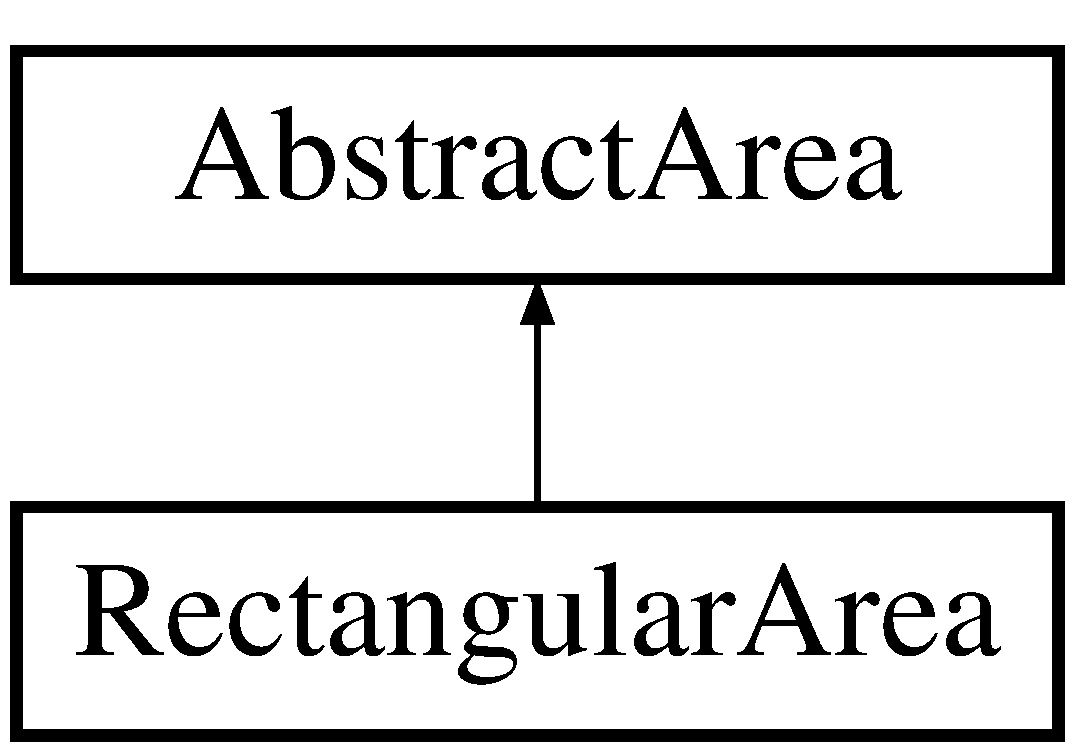
\includegraphics[height=2.000000cm]{class_abstract_area}
\end{center}
\end{figure}
\subsection*{Public Member Functions}
\begin{DoxyCompactItemize}
\item 
int \textbf{ get\+Dim} () const
\end{DoxyCompactItemize}
\subsection*{Protected Attributes}
\begin{DoxyCompactItemize}
\item 
\mbox{\label{class_abstract_area_a23e4a4c2637f2dca6aeeb4895d0d8735}} 
int {\bfseries dim}
\end{DoxyCompactItemize}


\subsection{Detailed Description}
Parent class for area in euclidian space. 

This class is used to represent abstract area in euclidian space of arbitrary dimension 

\subsection{Member Function Documentation}
\mbox{\label{class_abstract_area_a30ba3f8f1414674723061bee3bc7c0cc}} 
\index{Abstract\+Area@{Abstract\+Area}!get\+Dim@{get\+Dim}}
\index{get\+Dim@{get\+Dim}!Abstract\+Area@{Abstract\+Area}}
\subsubsection{get\+Dim()}
{\footnotesize\ttfamily int Abstract\+Area\+::get\+Dim (\begin{DoxyParamCaption}{ }\end{DoxyParamCaption}) const}

returns the dimension of an area 

The documentation for this class was generated from the following files\+:\begin{DoxyCompactItemize}
\item 
C\+:/\+Users/Владислав/\+Documents/\+Visual Studio 2015/\+Projects/local\+\_\+optimization/Abstract\+Area.\+h\item 
C\+:/\+Users/Владислав/\+Documents/\+Visual Studio 2015/\+Projects/local\+\_\+optimization/Abstract\+Area.\+cpp\end{DoxyCompactItemize}

\section{Abstract\+Function Class Reference}
\label{class_abstract_function}\index{Abstract\+Function@{Abstract\+Function}}
Inheritance diagram for Abstract\+Function\+:\begin{figure}[H]
\begin{center}
\leavevmode
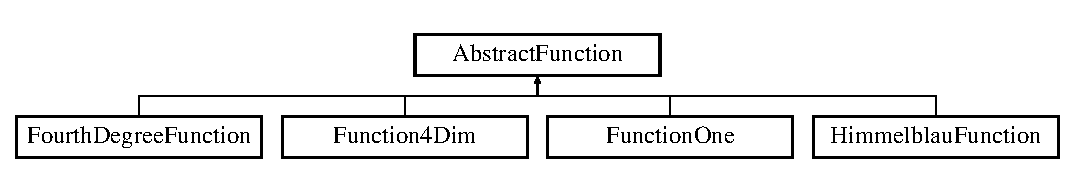
\includegraphics[height=1.891892cm]{class_abstract_function}
\end{center}
\end{figure}
\subsection*{Public Member Functions}
\begin{DoxyCompactItemize}
\item 
virtual double \textbf{ eval} (const Vector\+Xd \&x) const =0
\item 
\mbox{\label{class_abstract_function_a1e317092e346f8791c29fe468e364482}} 
virtual string {\bfseries get\+Name} ()=0
\item 
Vector\+Xd \textbf{ gradient} (const Vector\+Xd \&x) const
\item 
Matrix\+Xd \textbf{ hessian} (const Vector\+Xd \&x) const
\item 
int \textbf{ get\+Dim} () const
\item 
\textbf{ Rectangular\+Area} \textbf{ get\+Area} () const
\item 
void \textbf{ set\+Area} (const Vector\+Xd \&l, const Vector\+Xd \&r)
\end{DoxyCompactItemize}
\subsection*{Protected Attributes}
\begin{DoxyCompactItemize}
\item 
\mbox{\label{class_abstract_function_af31a6fcfa297e33f6e330ec4f85c8a40}} 
int {\bfseries dim}
\item 
\mbox{\label{class_abstract_function_ad19673268969e543d3871b15a0aba726}} 
bool {\bfseries is\+Convex}
\item 
\mbox{\label{class_abstract_function_ad8c7ab1978041adf814b8a8021e77823}} 
\textbf{ Rectangular\+Area} {\bfseries domain}
\end{DoxyCompactItemize}


\subsection{Member Function Documentation}
\mbox{\label{class_abstract_function_aff29a02b7083c1989c5e7dcf49312d31}} 
\index{Abstract\+Function@{Abstract\+Function}!eval@{eval}}
\index{eval@{eval}!Abstract\+Function@{Abstract\+Function}}
\subsubsection{eval()}
{\footnotesize\ttfamily virtual double Abstract\+Function\+::eval (\begin{DoxyParamCaption}\item[{const Vector\+Xd \&}]{x }\end{DoxyParamCaption}) const\hspace{0.3cm}{\ttfamily [pure virtual]}}

evaluates function at chosen vector 
\begin{DoxyParams}[1]{Parameters}
\mbox{\tt in}  & {\em x} & Vector of corresponding dimension \\
\hline
\end{DoxyParams}


Implemented in \textbf{ Function\+One} \doxyref{}{p.}{class_function_one_a27507eb602a2c520cdee4d6fd952d807}, \textbf{ Fourth\+Degree\+Function} \doxyref{}{p.}{class_fourth_degree_function_aa60e0ac44cc0ae5474bbabf92b20c7c1}, and \textbf{ Himmelblau\+Function} \doxyref{}{p.}{class_himmelblau_function_ae6aaab9b1087367128177f871d911855}.

\mbox{\label{class_abstract_function_a91976b6cc7078d37d1737d5cb6295f87}} 
\index{Abstract\+Function@{Abstract\+Function}!get\+Area@{get\+Area}}
\index{get\+Area@{get\+Area}!Abstract\+Function@{Abstract\+Function}}
\subsubsection{get\+Area()}
{\footnotesize\ttfamily \textbf{ Rectangular\+Area} Abstract\+Function\+::get\+Area (\begin{DoxyParamCaption}{ }\end{DoxyParamCaption}) const}

returns box domain of function \mbox{\label{class_abstract_function_a9f64864e3829c0993d939aadd28e9a45}} 
\index{Abstract\+Function@{Abstract\+Function}!get\+Dim@{get\+Dim}}
\index{get\+Dim@{get\+Dim}!Abstract\+Function@{Abstract\+Function}}
\subsubsection{get\+Dim()}
{\footnotesize\ttfamily int Abstract\+Function\+::get\+Dim (\begin{DoxyParamCaption}{ }\end{DoxyParamCaption}) const}

returns dimension \mbox{\label{class_abstract_function_acca8abaa171dee371a26630943069c21}} 
\index{Abstract\+Function@{Abstract\+Function}!gradient@{gradient}}
\index{gradient@{gradient}!Abstract\+Function@{Abstract\+Function}}
\subsubsection{gradient()}
{\footnotesize\ttfamily Vector\+Xd Abstract\+Function\+::gradient (\begin{DoxyParamCaption}\item[{const Vector\+Xd \&}]{x }\end{DoxyParamCaption}) const}

counts approximate gradient of a function at chosen vector 
\begin{DoxyParams}[1]{Parameters}
\mbox{\tt in}  & {\em x} & Vector of corresponding dimension \\
\hline
\end{DoxyParams}
\mbox{\label{class_abstract_function_aa13c89ccb1c6bb6f83691bac92a311f6}} 
\index{Abstract\+Function@{Abstract\+Function}!hessian@{hessian}}
\index{hessian@{hessian}!Abstract\+Function@{Abstract\+Function}}
\subsubsection{hessian()}
{\footnotesize\ttfamily Matrix\+Xd Abstract\+Function\+::hessian (\begin{DoxyParamCaption}\item[{const Vector\+Xd \&}]{x }\end{DoxyParamCaption}) const}

counts approximate hessian (matrix of second partial derivatives) at chosen vector 
\begin{DoxyParams}[1]{Parameters}
\mbox{\tt in}  & {\em x} & Vector of corresponding dimension \\
\hline
\end{DoxyParams}
\mbox{\label{class_abstract_function_ab9d67ef9caa1be5aefce762ec0f0016d}} 
\index{Abstract\+Function@{Abstract\+Function}!set\+Area@{set\+Area}}
\index{set\+Area@{set\+Area}!Abstract\+Function@{Abstract\+Function}}
\subsubsection{set\+Area()}
{\footnotesize\ttfamily void Abstract\+Function\+::set\+Area (\begin{DoxyParamCaption}\item[{const Vector\+Xd \&}]{l,  }\item[{const Vector\+Xd \&}]{r }\end{DoxyParamCaption})}

sets box domain of function 
\begin{DoxyParams}[1]{Parameters}
\mbox{\tt in}  & {\em l} & Vector of left borders \\
\hline
\mbox{\tt in}  & {\em r} & Vector of right borders \\
\hline
\end{DoxyParams}


The documentation for this class was generated from the following files\+:\begin{DoxyCompactItemize}
\item 
C\+:/\+Users/Владислав/\+Documents/\+Visual Studio 2015/\+Projects/local\+\_\+optimization/Abstract\+Function.\+h\item 
C\+:/\+Users/Владислав/\+Documents/\+Visual Studio 2015/\+Projects/local\+\_\+optimization/Abstract\+Function.\+cpp\end{DoxyCompactItemize}

\section{Abstract\+Optimizer Class Reference}
\label{class_abstract_optimizer}\index{Abstract\+Optimizer@{Abstract\+Optimizer}}
Inheritance diagram for Abstract\+Optimizer\+:\begin{figure}[H]
\begin{center}
\leavevmode
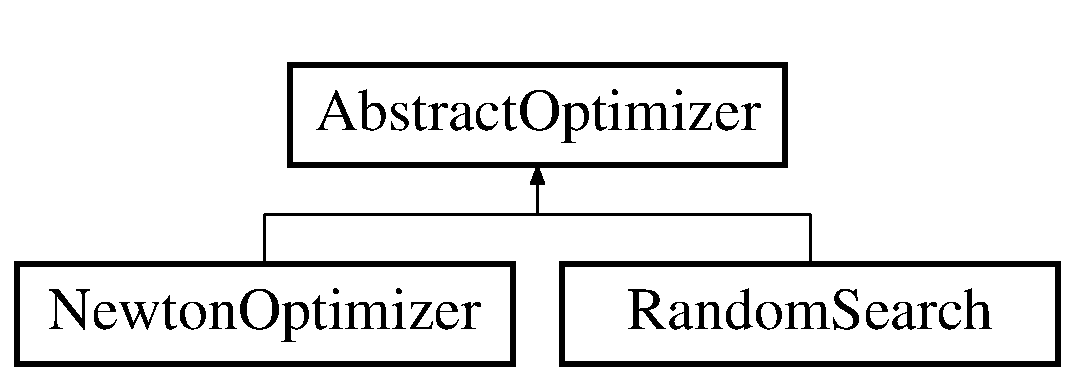
\includegraphics[height=2.000000cm]{class_abstract_optimizer}
\end{center}
\end{figure}
\subsection*{Protected Attributes}
\begin{DoxyCompactItemize}
\item 
\mbox{\label{class_abstract_optimizer_a200df06dc7a52d2c7ba97e26dad29025}} 
int {\bfseries dim}
\end{DoxyCompactItemize}


The documentation for this class was generated from the following files\+:\begin{DoxyCompactItemize}
\item 
C\+:/\+Users/Владислав/\+Documents/\+Visual Studio 2015/\+Projects/local\+\_\+optimization/Abstract\+Optimization.\+h\item 
C\+:/\+Users/Владислав/\+Documents/\+Visual Studio 2015/\+Projects/local\+\_\+optimization/Abstract\+Optimization.\+cpp\end{DoxyCompactItemize}

\section{Abstract\+Stop\+Crit Class Reference}
\label{class_abstract_stop_crit}\index{Abstract\+Stop\+Crit@{Abstract\+Stop\+Crit}}
Inheritance diagram for Abstract\+Stop\+Crit\+:\begin{figure}[H]
\begin{center}
\leavevmode
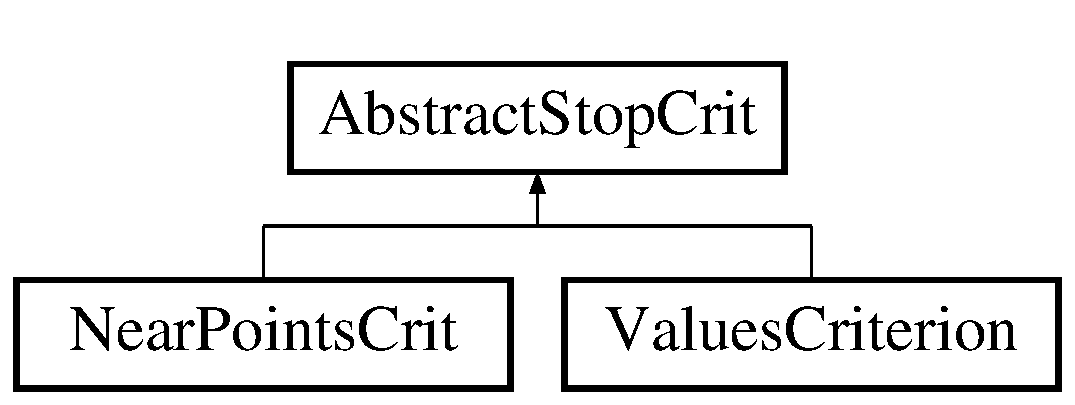
\includegraphics[height=2.000000cm]{class_abstract_stop_crit}
\end{center}
\end{figure}
\subsection*{Public Member Functions}
\begin{DoxyCompactItemize}
\item 
virtual bool \textbf{ criterion} (const Vector\+Xd \&x1, const Vector\+Xd \&x2, double eps, const \textbf{ Abstract\+Function} \&f) const =0
\end{DoxyCompactItemize}


\subsection{Member Function Documentation}
\mbox{\label{class_abstract_stop_crit_af4ac40006c2a60ae91865f4d1bb2aa94}} 
\index{Abstract\+Stop\+Crit@{Abstract\+Stop\+Crit}!criterion@{criterion}}
\index{criterion@{criterion}!Abstract\+Stop\+Crit@{Abstract\+Stop\+Crit}}
\subsubsection{criterion()}
{\footnotesize\ttfamily virtual bool Abstract\+Stop\+Crit\+::criterion (\begin{DoxyParamCaption}\item[{const Vector\+Xd \&}]{x1,  }\item[{const Vector\+Xd \&}]{x2,  }\item[{double}]{eps,  }\item[{const \textbf{ Abstract\+Function} \&}]{f }\end{DoxyParamCaption}) const\hspace{0.3cm}{\ttfamily [pure virtual]}}

compares two vectors and returns boolean value that stops optimization or not 
\begin{DoxyParams}[1]{Parameters}
\mbox{\tt in}  & {\em x1} & first vector \\
\hline
\mbox{\tt in}  & {\em x2} & second vector \\
\hline
\mbox{\tt in}  & {\em eps} & accuracy \\
\hline
\mbox{\tt in}  & {\em f} & function \\
\hline
\end{DoxyParams}


Implemented in \textbf{ Near\+Points\+Crit} \doxyref{}{p.}{class_near_points_crit_aadebf1f7eca578532c184ac91ab3322f}, and \textbf{ Values\+Criterion} \doxyref{}{p.}{class_values_criterion_a1277204c4e01db752b2031d2d6d60607}.



The documentation for this class was generated from the following files\+:\begin{DoxyCompactItemize}
\item 
C\+:/\+Users/Владислав/\+Documents/\+Visual Studio 2015/\+Projects/local\+\_\+optimization/Abstract\+Stop\+Crit.\+h\item 
C\+:/\+Users/Владислав/\+Documents/\+Visual Studio 2015/\+Projects/local\+\_\+optimization/Abstract\+Stop\+Crit.\+cpp\end{DoxyCompactItemize}

\section{Fourth\+Degree\+Function Class Reference}
\label{class_fourth_degree_function}\index{Fourth\+Degree\+Function@{Fourth\+Degree\+Function}}
Inheritance diagram for Fourth\+Degree\+Function\+:\begin{figure}[H]
\begin{center}
\leavevmode
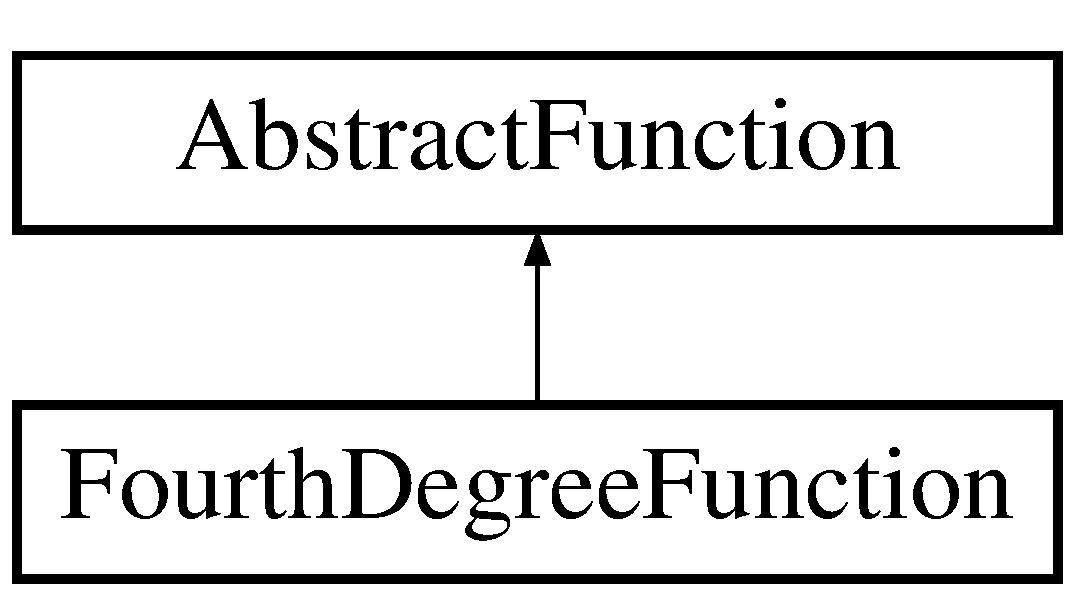
\includegraphics[height=2.000000cm]{class_fourth_degree_function}
\end{center}
\end{figure}
\subsection*{Public Member Functions}
\begin{DoxyCompactItemize}
\item 
\mbox{\label{class_fourth_degree_function_a5e42b52dc506629bb3d5a98a9be3daee}} 
string {\bfseries get\+Name} () override
\item 
double \textbf{ eval} (const Vector\+Xd \&x) const override
\end{DoxyCompactItemize}
\subsection*{Additional Inherited Members}


\subsection{Member Function Documentation}
\mbox{\label{class_fourth_degree_function_aa60e0ac44cc0ae5474bbabf92b20c7c1}} 
\index{Fourth\+Degree\+Function@{Fourth\+Degree\+Function}!eval@{eval}}
\index{eval@{eval}!Fourth\+Degree\+Function@{Fourth\+Degree\+Function}}
\subsubsection{eval()}
{\footnotesize\ttfamily double Fourth\+Degree\+Function\+::eval (\begin{DoxyParamCaption}\item[{const Vector\+Xd \&}]{x }\end{DoxyParamCaption}) const\hspace{0.3cm}{\ttfamily [override]}, {\ttfamily [virtual]}}

evaluates function at chosen vector 
\begin{DoxyParams}[1]{Parameters}
\mbox{\tt in}  & {\em x} & Vector of corresponding dimension \\
\hline
\end{DoxyParams}


Implements \textbf{ Abstract\+Function} \doxyref{}{p.}{class_abstract_function_aff29a02b7083c1989c5e7dcf49312d31}.



The documentation for this class was generated from the following files\+:\begin{DoxyCompactItemize}
\item 
C\+:/\+Users/Владислав/\+Documents/\+Visual Studio 2015/\+Projects/local\+\_\+optimization/Fourth\+Degree\+Function.\+h\item 
C\+:/\+Users/Владислав/\+Documents/\+Visual Studio 2015/\+Projects/local\+\_\+optimization/Fourth\+Degree\+Function.\+cpp\end{DoxyCompactItemize}

\section{Function4\+Dim Class Reference}
\label{class_function4_dim}\index{Function4\+Dim@{Function4\+Dim}}
Inheritance diagram for Function4\+Dim\+:\begin{figure}[H]
\begin{center}
\leavevmode
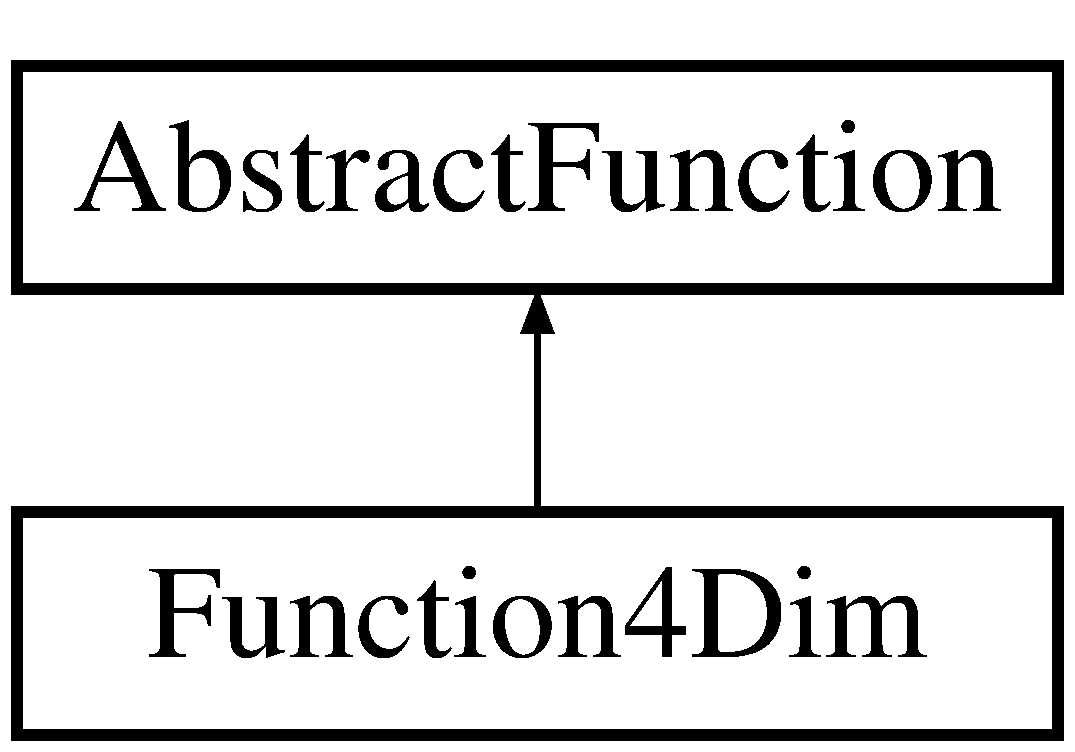
\includegraphics[height=2.000000cm]{class_function4_dim}
\end{center}
\end{figure}
\subsection*{Public Member Functions}
\begin{DoxyCompactItemize}
\item 
\mbox{\label{class_function4_dim_a7cfaeb2c4990cdac1d121bc516443dfe}} 
double {\bfseries eval} (const Eigen\+::\+Vector\+Xd \&x) const override
\item 
\mbox{\label{class_function4_dim_af54a4af564cca44274794581c66b271e}} 
{\bfseries Function4\+Dim} (const Vector\+Xd \&left, const Vector\+Xd \&right)
\end{DoxyCompactItemize}
\subsection*{Additional Inherited Members}


The documentation for this class was generated from the following files\+:\begin{DoxyCompactItemize}
\item 
C\+:/\+Users/Владислав/\+Documents/\+Visual Studio 2015/\+Projects/local\+\_\+optimization/Function4\+Dim.\+h\item 
C\+:/\+Users/Владислав/\+Documents/\+Visual Studio 2015/\+Projects/local\+\_\+optimization/Function4\+Dim.\+cpp\end{DoxyCompactItemize}

\section{Function\+One Class Reference}
\label{class_function_one}\index{Function\+One@{Function\+One}}
Inheritance diagram for Function\+One\+:\begin{figure}[H]
\begin{center}
\leavevmode
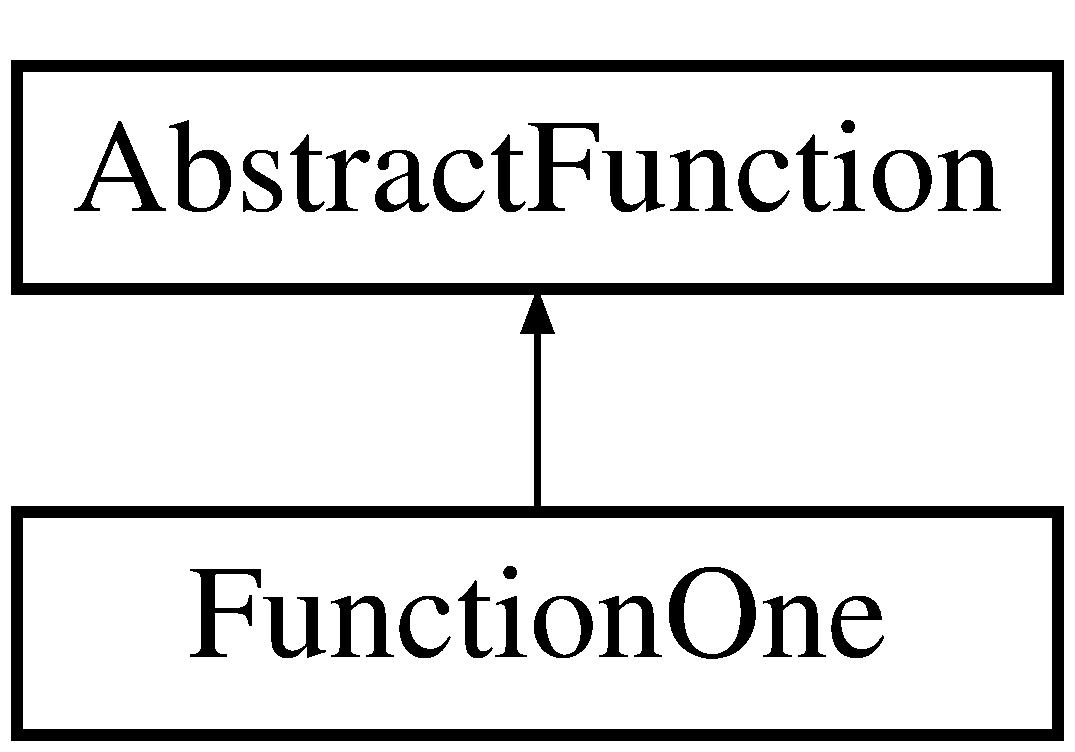
\includegraphics[height=2.000000cm]{class_function_one}
\end{center}
\end{figure}
\subsection*{Public Member Functions}
\begin{DoxyCompactItemize}
\item 
double \textbf{ eval} (const Vector\+Xd \&x) const override
\item 
\mbox{\label{class_function_one_afb28502596849eb13040121f02c9e16c}} 
string {\bfseries get\+Name} () override
\end{DoxyCompactItemize}
\subsection*{Additional Inherited Members}


\subsection{Member Function Documentation}
\mbox{\label{class_function_one_a27507eb602a2c520cdee4d6fd952d807}} 
\index{Function\+One@{Function\+One}!eval@{eval}}
\index{eval@{eval}!Function\+One@{Function\+One}}
\subsubsection{eval()}
{\footnotesize\ttfamily double Function\+One\+::eval (\begin{DoxyParamCaption}\item[{const Vector\+Xd \&}]{x }\end{DoxyParamCaption}) const\hspace{0.3cm}{\ttfamily [override]}, {\ttfamily [virtual]}}

evaluates function at chosen vector 
\begin{DoxyParams}[1]{Parameters}
\mbox{\tt in}  & {\em x} & Vector of corresponding dimension \\
\hline
\end{DoxyParams}


Implements \textbf{ Abstract\+Function} \doxyref{}{p.}{class_abstract_function_aff29a02b7083c1989c5e7dcf49312d31}.



The documentation for this class was generated from the following files\+:\begin{DoxyCompactItemize}
\item 
C\+:/\+Users/Владислав/\+Documents/\+Visual Studio 2015/\+Projects/local\+\_\+optimization/Function\+One.\+h\item 
C\+:/\+Users/Владислав/\+Documents/\+Visual Studio 2015/\+Projects/local\+\_\+optimization/Function\+One.\+cpp\end{DoxyCompactItemize}

\section{Himmelblau\+Function Class Reference}
\label{class_himmelblau_function}\index{Himmelblau\+Function@{Himmelblau\+Function}}
Inheritance diagram for Himmelblau\+Function\+:\begin{figure}[H]
\begin{center}
\leavevmode
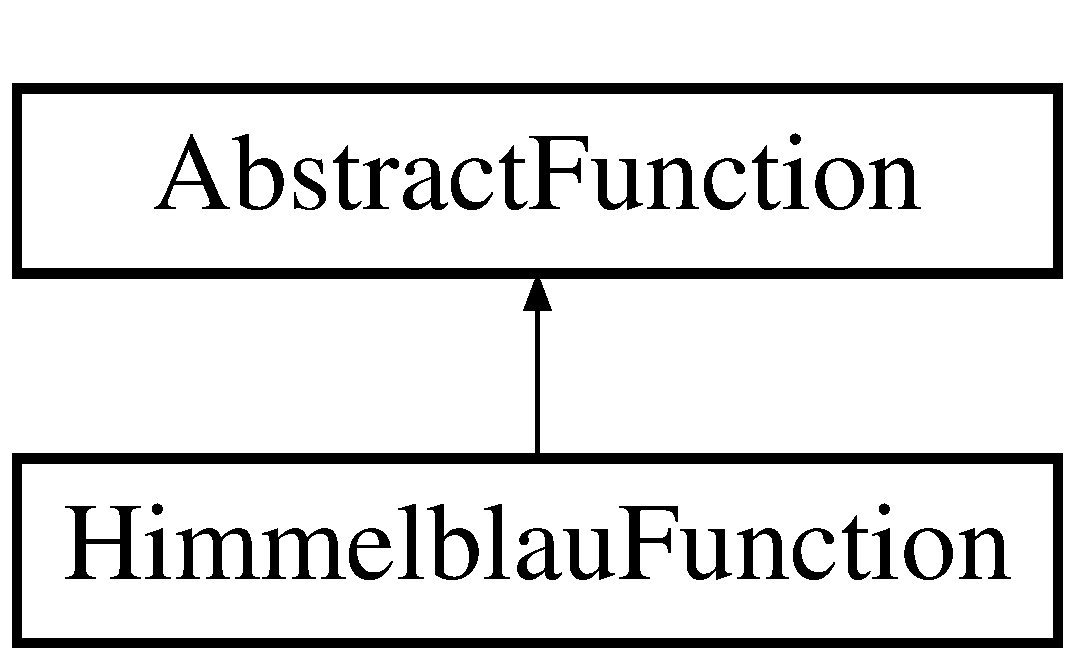
\includegraphics[height=2.000000cm]{class_himmelblau_function}
\end{center}
\end{figure}
\subsection*{Public Member Functions}
\begin{DoxyCompactItemize}
\item 
\mbox{\label{class_himmelblau_function_aca28aa62f0711c72dd31cf019f38ca20}} 
string {\bfseries get\+Name} () override
\item 
double \textbf{ eval} (const Vector\+Xd \&x) const override
\end{DoxyCompactItemize}
\subsection*{Additional Inherited Members}


\subsection{Member Function Documentation}
\mbox{\label{class_himmelblau_function_ae6aaab9b1087367128177f871d911855}} 
\index{Himmelblau\+Function@{Himmelblau\+Function}!eval@{eval}}
\index{eval@{eval}!Himmelblau\+Function@{Himmelblau\+Function}}
\subsubsection{eval()}
{\footnotesize\ttfamily double Himmelblau\+Function\+::eval (\begin{DoxyParamCaption}\item[{const Vector\+Xd \&}]{x }\end{DoxyParamCaption}) const\hspace{0.3cm}{\ttfamily [override]}, {\ttfamily [virtual]}}

evaluates function at chosen vector 
\begin{DoxyParams}[1]{Parameters}
\mbox{\tt in}  & {\em x} & Vector of corresponding dimension \\
\hline
\end{DoxyParams}


Implements \textbf{ Abstract\+Function} \doxyref{}{p.}{class_abstract_function_aff29a02b7083c1989c5e7dcf49312d31}.



The documentation for this class was generated from the following files\+:\begin{DoxyCompactItemize}
\item 
C\+:/\+Users/Владислав/\+Documents/\+Visual Studio 2015/\+Projects/local\+\_\+optimization/Himmelblau\+Function.\+h\item 
C\+:/\+Users/Владислав/\+Documents/\+Visual Studio 2015/\+Projects/local\+\_\+optimization/Himmelblau\+Function.\+cpp\end{DoxyCompactItemize}

\section{Near\+Points\+Crit Class Reference}
\label{class_near_points_crit}\index{Near\+Points\+Crit@{Near\+Points\+Crit}}


Stop criterion.  




{\ttfamily \#include $<$Near\+Points\+Crit.\+h$>$}

Inheritance diagram for Near\+Points\+Crit\+:\begin{figure}[H]
\begin{center}
\leavevmode
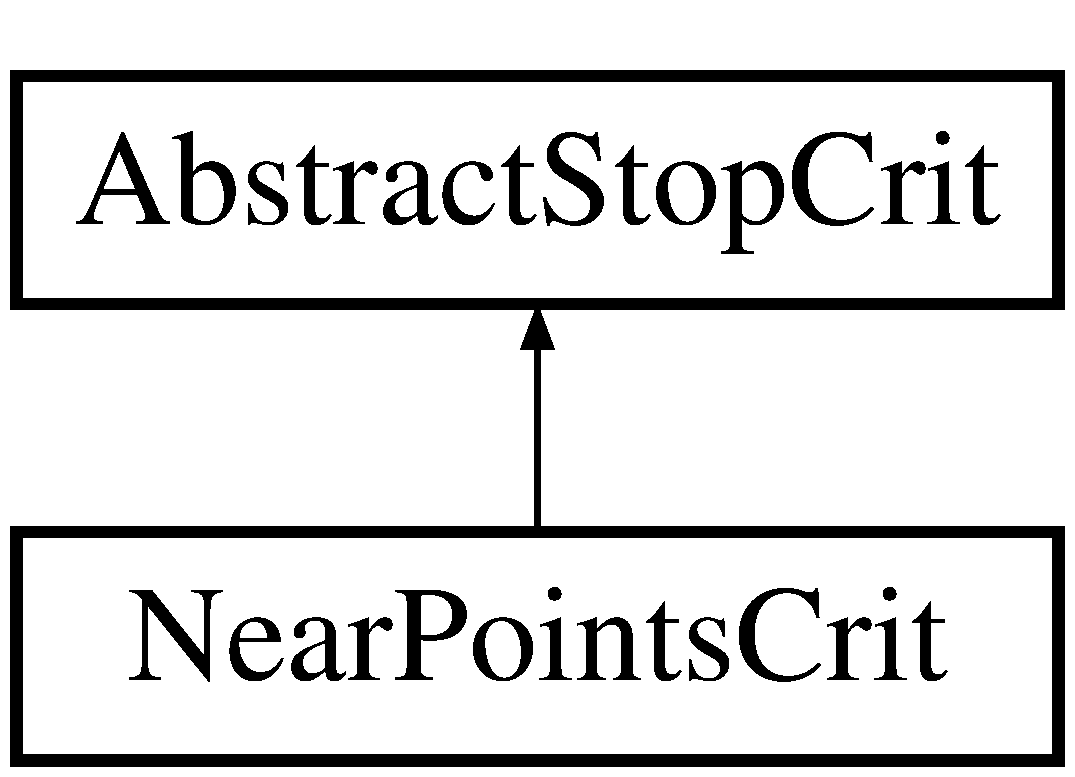
\includegraphics[height=2.000000cm]{class_near_points_crit}
\end{center}
\end{figure}
\subsection*{Public Member Functions}
\begin{DoxyCompactItemize}
\item 
bool \textbf{ criterion} (const Vector\+Xd \&x1, const Vector\+Xd \&x2, double eps, const \textbf{ Abstract\+Function} \&f) const override
\end{DoxyCompactItemize}


\subsection{Detailed Description}
Stop criterion. 

Stop criterion that compares how near are two iterations. Extends \doxyref{Abstract\+Stop\+Crit}{p.}{class_abstract_stop_crit} 

\subsection{Member Function Documentation}
\mbox{\label{class_near_points_crit_aadebf1f7eca578532c184ac91ab3322f}} 
\index{Near\+Points\+Crit@{Near\+Points\+Crit}!criterion@{criterion}}
\index{criterion@{criterion}!Near\+Points\+Crit@{Near\+Points\+Crit}}
\subsubsection{criterion()}
{\footnotesize\ttfamily bool Near\+Points\+Crit\+::criterion (\begin{DoxyParamCaption}\item[{const Vector\+Xd \&}]{x1,  }\item[{const Vector\+Xd \&}]{x2,  }\item[{double}]{eps,  }\item[{const \textbf{ Abstract\+Function} \&}]{f }\end{DoxyParamCaption}) const\hspace{0.3cm}{\ttfamily [override]}, {\ttfamily [virtual]}}

compares two vectors and returns boolean value that stops optimization or not 
\begin{DoxyParams}[1]{Parameters}
\mbox{\tt in}  & {\em x1} & first vector \\
\hline
\mbox{\tt in}  & {\em x2} & second vector \\
\hline
\mbox{\tt in}  & {\em eps} & accuracy \\
\hline
\mbox{\tt in}  & {\em f} & function \\
\hline
\end{DoxyParams}


Implements \textbf{ Abstract\+Stop\+Crit} \doxyref{}{p.}{class_abstract_stop_crit_af4ac40006c2a60ae91865f4d1bb2aa94}.



The documentation for this class was generated from the following files\+:\begin{DoxyCompactItemize}
\item 
C\+:/\+Users/Владислав/\+Documents/\+Visual Studio 2015/\+Projects/local\+\_\+optimization/Near\+Points\+Crit.\+h\item 
C\+:/\+Users/Владислав/\+Documents/\+Visual Studio 2015/\+Projects/local\+\_\+optimization/Near\+Points\+Crit.\+cpp\end{DoxyCompactItemize}

\section{Newton\+Optimizer Class Reference}
\label{class_newton_optimizer}\index{Newton\+Optimizer@{Newton\+Optimizer}}


Newton method.  




{\ttfamily \#include $<$Newton\+Optimizer.\+h$>$}

Inheritance diagram for Newton\+Optimizer\+:\begin{figure}[H]
\begin{center}
\leavevmode
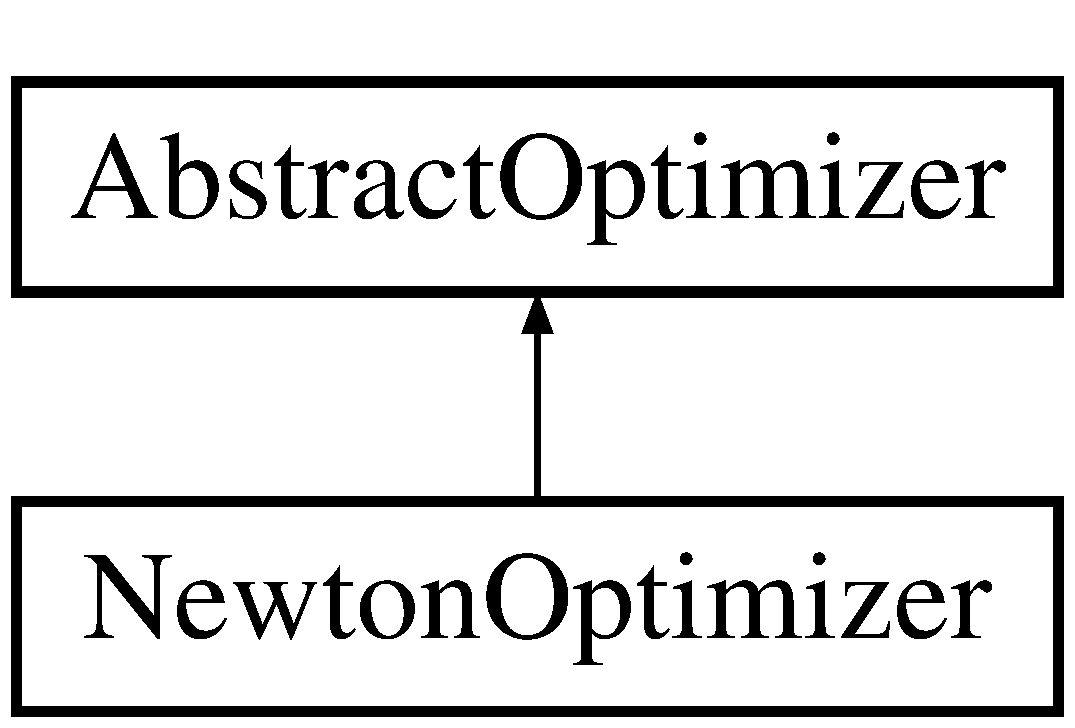
\includegraphics[height=2.000000cm]{class_newton_optimizer}
\end{center}
\end{figure}
\subsection*{Public Member Functions}
\begin{DoxyCompactItemize}
\item 
Vector\+Xd \textbf{ optim} (const Vector\+Xd \&x0, double eps, const \textbf{ Abstract\+Function} \&f, const \textbf{ Abstract\+Stop\+Crit} \&stop) const
\end{DoxyCompactItemize}
\subsection*{Additional Inherited Members}


\subsection{Detailed Description}
Newton method. 

Class that provides optimization with newton method. Extends \doxyref{Abstract\+Optimizer}{p.}{class_abstract_optimizer} 

\subsection{Member Function Documentation}
\mbox{\label{class_newton_optimizer_a41905879dac33770e0bd3943d5ea469f}} 
\index{Newton\+Optimizer@{Newton\+Optimizer}!optim@{optim}}
\index{optim@{optim}!Newton\+Optimizer@{Newton\+Optimizer}}
\subsubsection{optim()}
{\footnotesize\ttfamily Vector\+Xd Newton\+Optimizer\+::optim (\begin{DoxyParamCaption}\item[{const Vector\+Xd \&}]{x0,  }\item[{double}]{eps,  }\item[{const \textbf{ Abstract\+Function} \&}]{f,  }\item[{const \textbf{ Abstract\+Stop\+Crit} \&}]{stop }\end{DoxyParamCaption}) const}

performs local optimization using Newton method. Returns argument of local minimum 
\begin{DoxyParams}[1]{Parameters}
\mbox{\tt in}  & {\em x0} & initial vector \\
\hline
\mbox{\tt in}  & {\em eps} & accuracy \\
\hline
\mbox{\tt in}  & {\em f} & function \\
\hline
\mbox{\tt in}  & {\em stop} & Stop criterion \\
\hline
\end{DoxyParams}


The documentation for this class was generated from the following files\+:\begin{DoxyCompactItemize}
\item 
C\+:/\+Users/Владислав/\+Documents/\+Visual Studio 2015/\+Projects/local\+\_\+optimization/Newton\+Optimizer.\+h\item 
C\+:/\+Users/Владислав/\+Documents/\+Visual Studio 2015/\+Projects/local\+\_\+optimization/Newton\+Optimizer.\+cpp\end{DoxyCompactItemize}

\section{Random\+Search Class Reference}
\label{class_random_search}\index{Random\+Search@{Random\+Search}}
Inheritance diagram for Random\+Search\+:\begin{figure}[H]
\begin{center}
\leavevmode
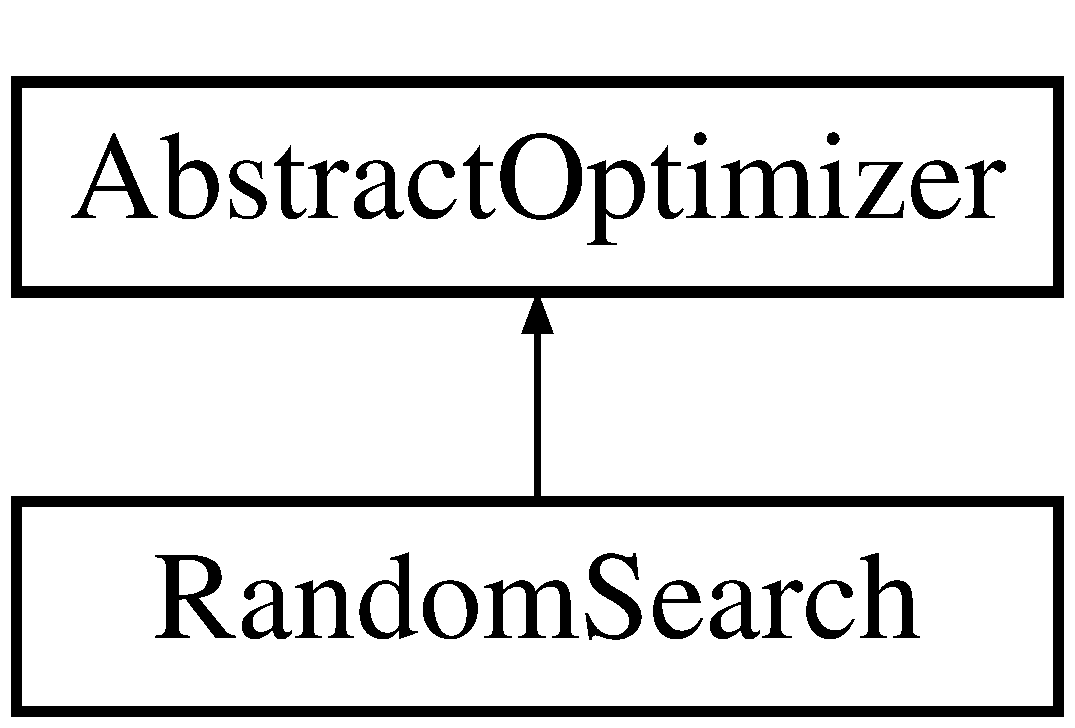
\includegraphics[height=2.000000cm]{class_random_search}
\end{center}
\end{figure}
\subsection*{Public Member Functions}
\begin{DoxyCompactItemize}
\item 
Vector\+Xd \textbf{ optim} (const \textbf{ Abstract\+Function} \&f)
\item 
Vector\+Xd \textbf{ get\+Point\+In\+Area} (const \textbf{ Rectangular\+Area} \&area)
\item 
\mbox{\label{class_random_search_a3158fb489b681187d450c5297b90ce84}} 
{\bfseries Random\+Search} (double prob)
\end{DoxyCompactItemize}
\subsection*{Additional Inherited Members}


\subsection{Member Function Documentation}
\mbox{\label{class_random_search_a5f7910c44bb6a57851a01fb0a868ba8c}} 
\index{Random\+Search@{Random\+Search}!get\+Point\+In\+Area@{get\+Point\+In\+Area}}
\index{get\+Point\+In\+Area@{get\+Point\+In\+Area}!Random\+Search@{Random\+Search}}
\subsubsection{get\+Point\+In\+Area()}
{\footnotesize\ttfamily Vector\+Xd Random\+Search\+::get\+Point\+In\+Area (\begin{DoxyParamCaption}\item[{const \textbf{ Rectangular\+Area} \&}]{area }\end{DoxyParamCaption})}

gets random uniformly distributed point in an area 
\begin{DoxyParams}[1]{Parameters}
\mbox{\tt in}  & {\em area} & box area \\
\hline
\end{DoxyParams}
\mbox{\label{class_random_search_a2b8ff71f70232639f87a71e22d63edaf}} 
\index{Random\+Search@{Random\+Search}!optim@{optim}}
\index{optim@{optim}!Random\+Search@{Random\+Search}}
\subsubsection{optim()}
{\footnotesize\ttfamily Vector\+Xd Random\+Search\+::optim (\begin{DoxyParamCaption}\item[{const \textbf{ Abstract\+Function} \&}]{f }\end{DoxyParamCaption})}

performs random search to find global minimum 
\begin{DoxyParams}[1]{Parameters}
\mbox{\tt in}  & {\em f} & function to optimize \\
\hline
\end{DoxyParams}


The documentation for this class was generated from the following files\+:\begin{DoxyCompactItemize}
\item 
C\+:/\+Users/Владислав/\+Documents/\+Visual Studio 2015/\+Projects/local\+\_\+optimization/Random\+Search.\+h\item 
C\+:/\+Users/Владислав/\+Documents/\+Visual Studio 2015/\+Projects/local\+\_\+optimization/Random\+Search.\+cpp\end{DoxyCompactItemize}

\section{Rectangular\+Area Class Reference}
\label{class_rectangular_area}\index{Rectangular\+Area@{Rectangular\+Area}}
Inheritance diagram for Rectangular\+Area\+:\begin{figure}[H]
\begin{center}
\leavevmode
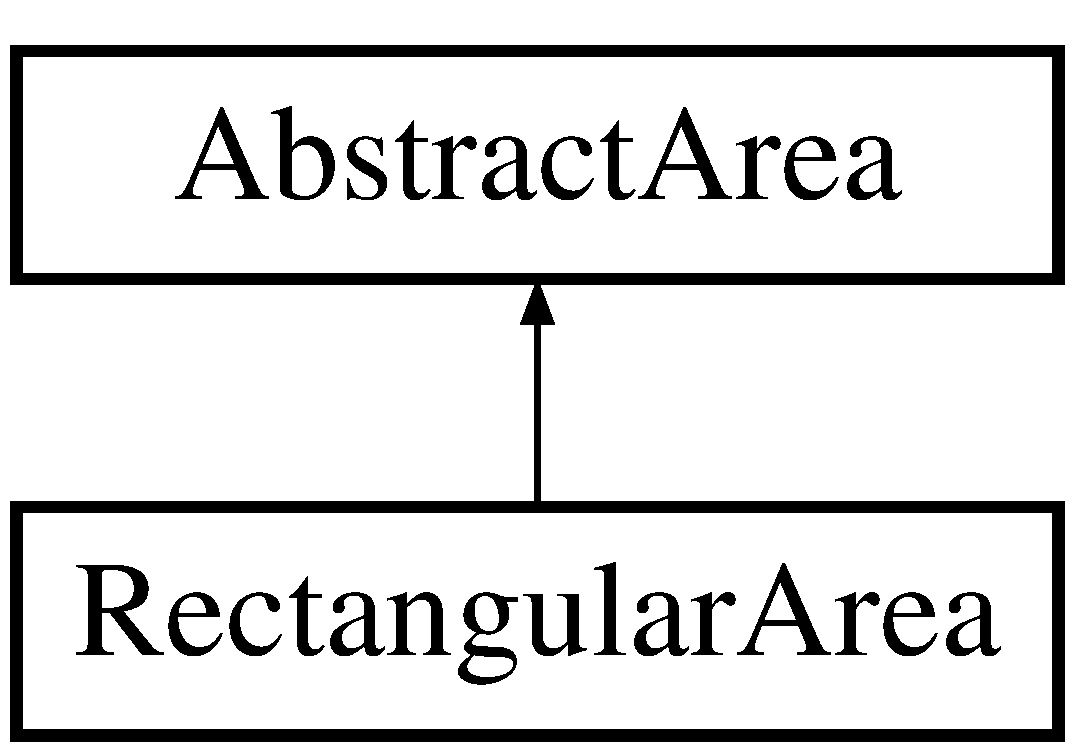
\includegraphics[height=2.000000cm]{class_rectangular_area}
\end{center}
\end{figure}
\subsection*{Public Member Functions}
\begin{DoxyCompactItemize}
\item 
Vector\+Xd \textbf{ get\+Left} () const
\item 
Vector\+Xd \textbf{ get\+Right} () const
\item 
\mbox{\label{class_rectangular_area_a24391dafbb67092f7670b40f5e10508f}} 
{\bfseries Rectangular\+Area} (const Vector\+Xd \&l, const Vector\+Xd \&r, int d)
\end{DoxyCompactItemize}
\subsection*{Additional Inherited Members}


\subsection{Member Function Documentation}
\mbox{\label{class_rectangular_area_a1e1c3de69c38826425015ce56b2db72b}} 
\index{Rectangular\+Area@{Rectangular\+Area}!get\+Left@{get\+Left}}
\index{get\+Left@{get\+Left}!Rectangular\+Area@{Rectangular\+Area}}
\subsubsection{get\+Left()}
{\footnotesize\ttfamily Vector\+Xd Rectangular\+Area\+::get\+Left (\begin{DoxyParamCaption}{ }\end{DoxyParamCaption}) const}

gets vector of left borders \mbox{\label{class_rectangular_area_a1c8b68b80a6e15f1ee879db1166910b6}} 
\index{Rectangular\+Area@{Rectangular\+Area}!get\+Right@{get\+Right}}
\index{get\+Right@{get\+Right}!Rectangular\+Area@{Rectangular\+Area}}
\subsubsection{get\+Right()}
{\footnotesize\ttfamily Vector\+Xd Rectangular\+Area\+::get\+Right (\begin{DoxyParamCaption}{ }\end{DoxyParamCaption}) const}

gets vector of right borders 

The documentation for this class was generated from the following files\+:\begin{DoxyCompactItemize}
\item 
C\+:/\+Users/Владислав/\+Documents/\+Visual Studio 2015/\+Projects/local\+\_\+optimization/Rectangular\+Area.\+h\item 
C\+:/\+Users/Владислав/\+Documents/\+Visual Studio 2015/\+Projects/local\+\_\+optimization/Rectangular\+Area.\+cpp\end{DoxyCompactItemize}

\section{Values\+Criterion Class Reference}
\label{class_values_criterion}\index{Values\+Criterion@{Values\+Criterion}}


{\ttfamily \#include $<$Values\+Criterion.\+h$>$}

Inheritance diagram for Values\+Criterion\+:\begin{figure}[H]
\begin{center}
\leavevmode
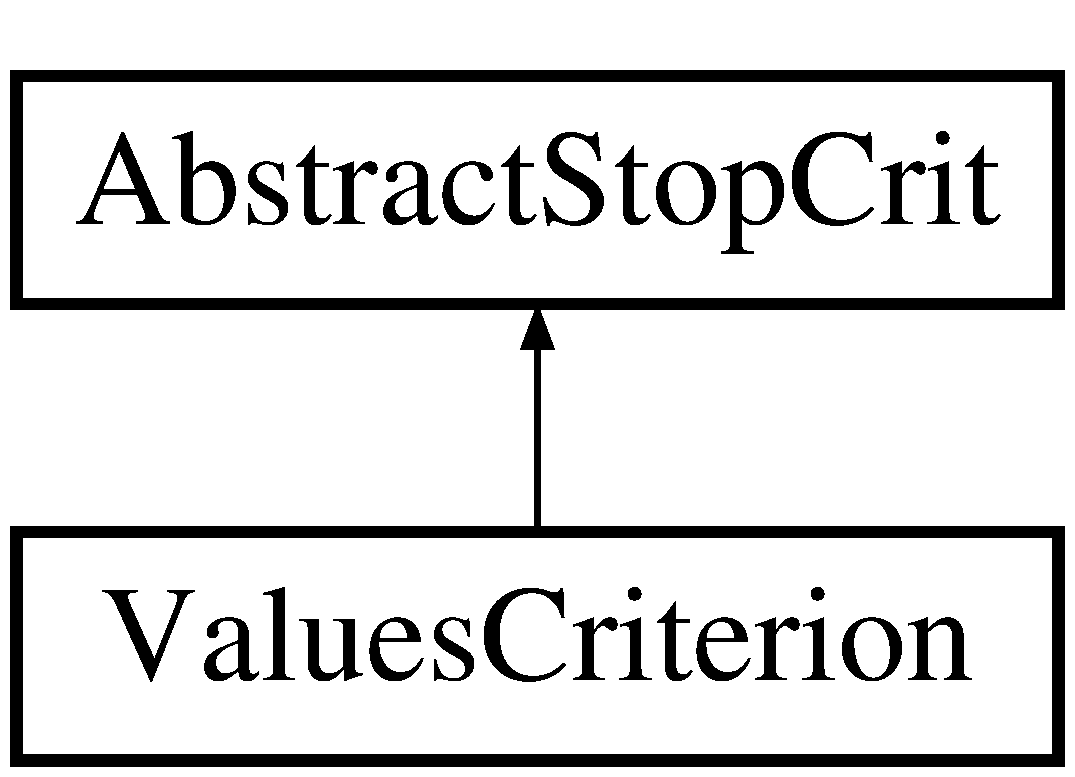
\includegraphics[height=2.000000cm]{class_values_criterion}
\end{center}
\end{figure}
\subsection*{Public Member Functions}
\begin{DoxyCompactItemize}
\item 
bool \textbf{ criterion} (const Vector\+Xd \&x1, const Vector\+Xd \&x2, double eps, const \textbf{ Abstract\+Function} \&f) const
\end{DoxyCompactItemize}


\subsection{Detailed Description}
stop criterion that checks how near are values of function in two vectors 

\subsection{Member Function Documentation}
\mbox{\label{class_values_criterion_a1277204c4e01db752b2031d2d6d60607}} 
\index{Values\+Criterion@{Values\+Criterion}!criterion@{criterion}}
\index{criterion@{criterion}!Values\+Criterion@{Values\+Criterion}}
\subsubsection{criterion()}
{\footnotesize\ttfamily bool Values\+Criterion\+::criterion (\begin{DoxyParamCaption}\item[{const Vector\+Xd \&}]{x1,  }\item[{const Vector\+Xd \&}]{x2,  }\item[{double}]{eps,  }\item[{const \textbf{ Abstract\+Function} \&}]{f }\end{DoxyParamCaption}) const\hspace{0.3cm}{\ttfamily [virtual]}}

compares two vectors and returns boolean value that stops optimization or not 
\begin{DoxyParams}[1]{Parameters}
\mbox{\tt in}  & {\em x1} & first vector \\
\hline
\mbox{\tt in}  & {\em x2} & second vector \\
\hline
\mbox{\tt in}  & {\em eps} & accuracy \\
\hline
\mbox{\tt in}  & {\em f} & function \\
\hline
\end{DoxyParams}


Implements \textbf{ Abstract\+Stop\+Crit} \doxyref{}{p.}{class_abstract_stop_crit_af4ac40006c2a60ae91865f4d1bb2aa94}.



The documentation for this class was generated from the following files\+:\begin{DoxyCompactItemize}
\item 
C\+:/\+Users/Владислав/\+Documents/\+Visual Studio 2015/\+Projects/local\+\_\+optimization/Values\+Criterion.\+h\item 
C\+:/\+Users/Владислав/\+Documents/\+Visual Studio 2015/\+Projects/local\+\_\+optimization/Values\+Criterion.\+cpp\end{DoxyCompactItemize}

\chapter{File Documentation}
\section{C\+:/\+Users/Владислав/\+Documents/\+Visual Studio 2015/\+Projects/local\+\_\+optimization/\+Values.h File Reference}
\label{_values_8h}\index{C\+:/\+Users/Владислав/\+Documents/\+Visual Studio 2015/\+Projects/local\+\_\+optimization/\+Values.\+h@{C\+:/\+Users/Владислав/\+Documents/\+Visual Studio 2015/\+Projects/local\+\_\+optimization/\+Values.\+h}}


Header file that contains default constant values.  


\subsection*{Variables}
\begin{DoxyCompactItemize}
\item 
\mbox{\label{_values_8h_a596344e5a2992d2beec43b76a6294de0}} 
const double {\bfseries E\+P\+S\+I\+L\+ON} = 0.\+00001
\item 
\mbox{\label{_values_8h_ac398e4bea943a72137f06ff1146e65b7}} 
const int {\bfseries M\+A\+X\+\_\+\+I\+T\+E\+R\+A\+T\+I\+O\+NS} = 50000
\item 
\mbox{\label{_values_8h_a5b739a927874790745d45a63f7fc8fa4}} 
const int {\bfseries C\+O\+U\+N\+T\+\_\+\+S\+U\+C\+C\+E\+S\+S\+ES} = 100
\item 
\mbox{\label{_values_8h_a2ce13072b971784cb5bce4712cff4c3d}} 
const double {\bfseries S\+T\+EP} = 0.\+01
\item 
\mbox{\label{_values_8h_acd9d397749ce2ed992cc4ee45108475f}} 
const string {\bfseries R\+O\+S\+E\+N\+B\+R\+O\+C\+K\+\_\+\+F\+U\+N\+C\+T\+I\+ON} = \char`\"{}100 $\ast$ (x(1) -\/ x(0) $\ast$ x(0))$\ast$(x(1) -\/ x(0) $\ast$ x(0)) + (1 -\/ x(0)) $\ast$ (1 -\/ x(0)) (Non-\/convex)\char`\"{}
\item 
\mbox{\label{_values_8h_adc4aeb3ae8f2805ba8ab966847e2a94b}} 
const string {\bfseries H\+I\+M\+M\+E\+L\+B\+L\+A\+U\+\_\+\+F\+U\+N\+C\+T\+I\+ON} = \char`\"{}((x(0)$\ast$x(0) + x(1) -\/ 11)$\ast$(x(0)$\ast$x(0) + x(1) -\/ 11) + (x(0) + x(1)$\ast$x(1) -\/ 7)$\ast$(x(0) + x(1)$\ast$x(1) -\/ 7)) (Non-\/convex)\char`\"{}
\item 
\mbox{\label{_values_8h_a067b30858917621cd28972c4517967af}} 
const string {\bfseries F\+O\+U\+R\+T\+H\+\_\+\+D\+E\+G\+R\+E\+E\+\_\+\+F\+U\+N\+C\+T\+I\+ON} = \char`\"{}(x(0)$\ast$x(0)$\ast$x(0)$\ast$x(0) + x(1)$\ast$x(1)$\ast$x(1)$\ast$x(1)) (Convex)\char`\"{}
\end{DoxyCompactItemize}


\subsection{Detailed Description}
Header file that contains default constant values. 

This file contains constant values that are used in program 
%--- End generated contents ---

% Index
\backmatter
\newpage
\phantomsection
\clearemptydoublepage
\addcontentsline{toc}{chapter}{Index}
\printindex

\end{document}
